\chapter{Results and interpretation}\label{chap:results}
Now that all backgrounds are well estimated, the background prediction seems to work fine in te validation region, and all uncertainties are determined, the background prediction can be applied to the SR, $\ptmiss>150\GeV$ and $\mtTwo>100\GeV$, and predicted and observed event counts can be compared. An excess or other significant deviations from the prediction would be indicators for BSM physics.
\section{Results}\label{sec:results}
\subsection*{Signal region binning}
In order to perform the counting experiment, a distinct binning in one or multiple variables needs to be applied to the SR. This binning can be optimized considering different criteria, \eg observation and exlcusion power. Since the most sensitive variables are $\ptmiss$ and $\mtTwo$, different one dimensional and two dimensional binnings were tried. Therefore, for individual benchmark points of all three signal models, simplified significances $\frac{s}{s+b}$, where s is the number of signal events and b the number of backgground events per bin, the binnings are varied. Because the total predicted event count in the SR is of the order of $13$ events, special care hast to be taken regarding this issue. Albeit many sensitive bins with lower SM prediction and high signal expectation would push expected exclusion limits, this would make reinterpretations and observaions difficult due to the high statistical uncertainties on the measured data.\\
To take into consideraton all those issues, a binning consisting of two bins in the $\ptmiss$ miss distribution are chosen, as already introduced in \refSec{sec:SRSelection}. The first bin starts at $150\GeV$ and ends at $200\GeV$, while the second one is an overflow bin, meaning all events with $\ptmiss>200\GeV$ in the SR are counted in that bin. This binning yields on the one side good exclusion power because the $\ptmiss$ distribution is observed to be more sensitive than the $\mtTwo$ distribution, and on the other side has an amount of events large enough in each bin, that the measurement is not limited by statistical uncertainties. Due to the same reasons two dimensional binnings are discarded.
\subsubsection*{Possible influence of signal to the validation region}
The SR and the VR are very close to each other in phasespace due to the chosen sideband structure of the VR. Thus, some signal events, especially for low SUSY masses, are expected to populate also the VR. The most sensitive distribution to this effect is the $\pt$ distribution of the selected photon, as shown in \refFig{fig:signalContVR}.
\begin{figure}[tbp]
 \centering
 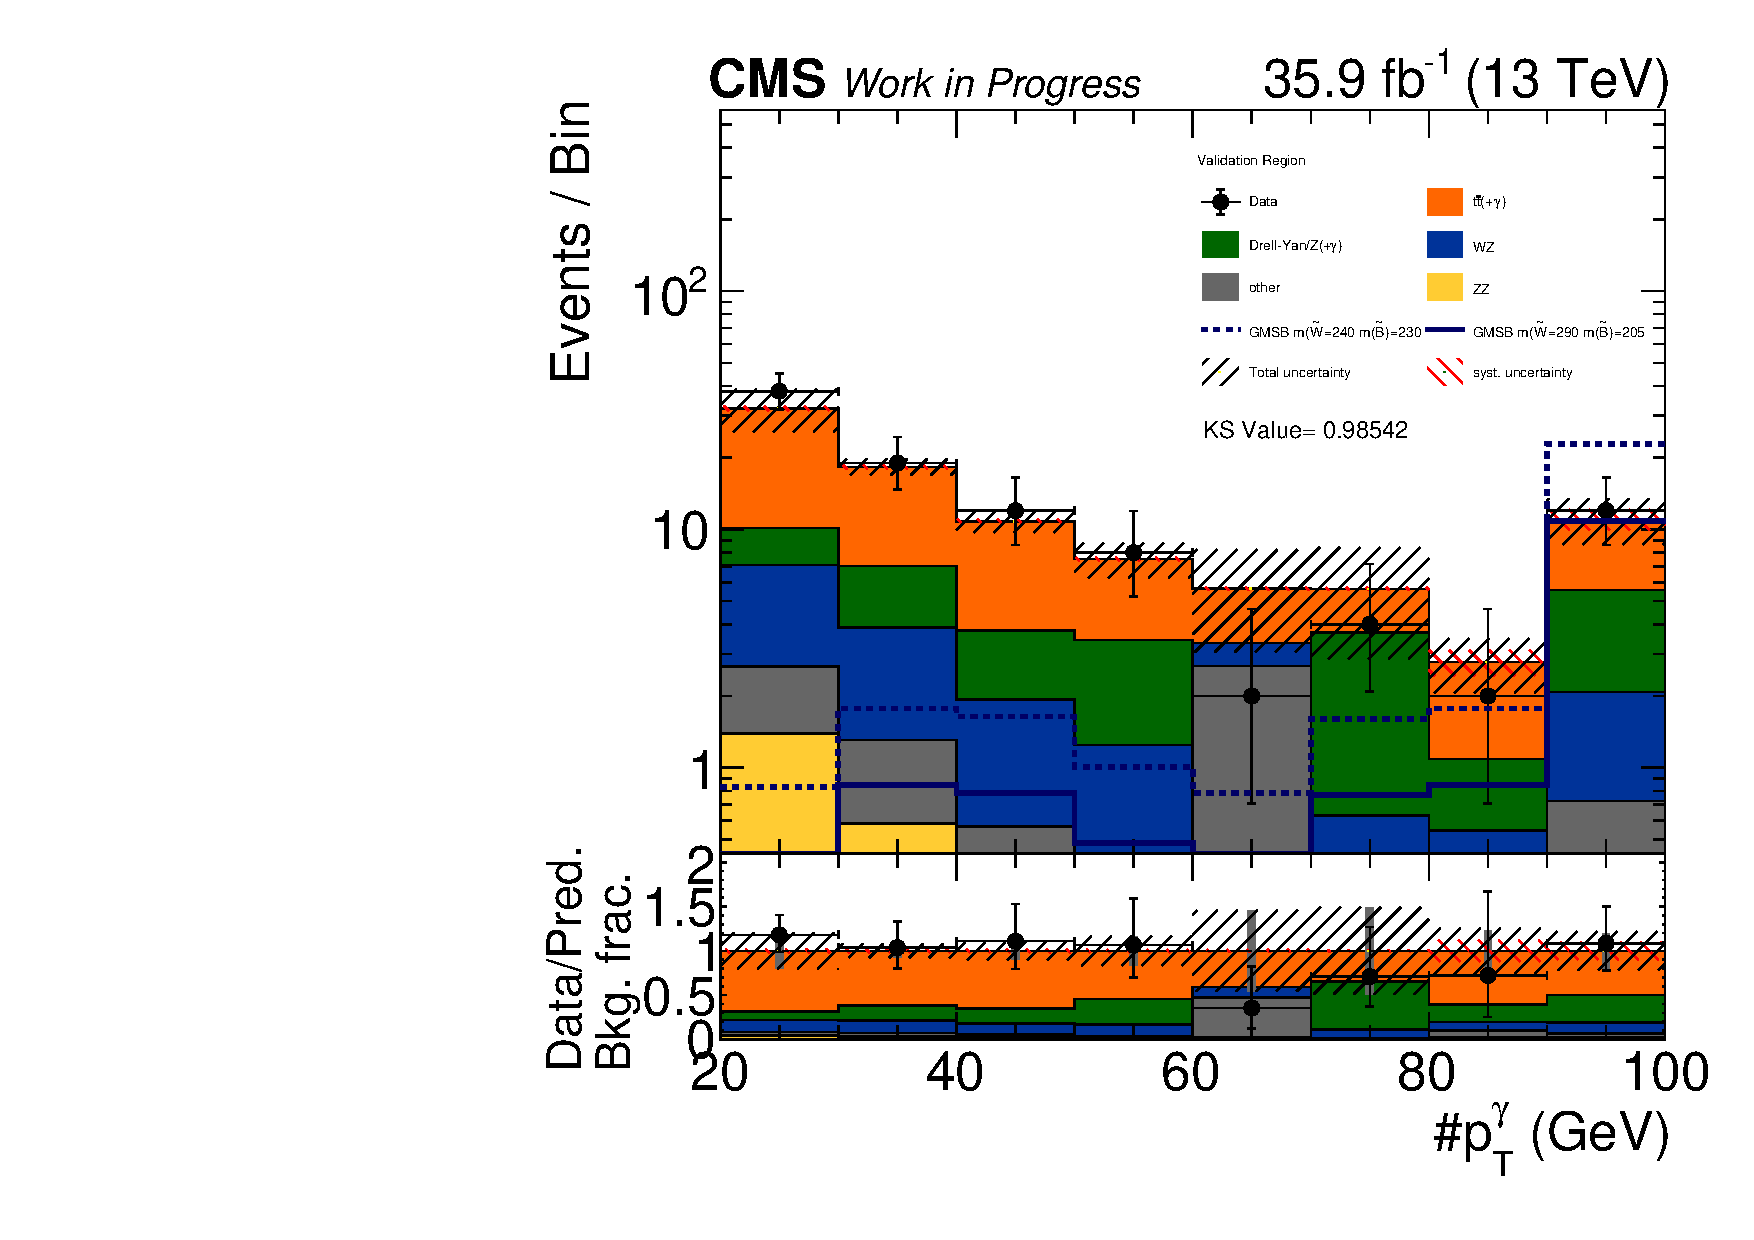
\includegraphics[width=\pairwidth]{figures/VR_signal_study/VR_LL_pt_g1_log}
 \caption{todo}
 \label{fig:signalContVR}
\end{figure}
At high $\pt^{\PGg}$ ranges ($>80\GeV$), a considerable amount of signal events is measurable in the VR. Since the predicted background and observed data are already compared in the VR, and no background prediction is performed here, there is no need to account for this effect like in the other CR in terms of signal contamination.\\
Hence, the subtraction of this region and the addition of adding it to the SR as a third search bin would increase the total sensitivity. But, because the number of expeed signal events in the two SR bins is  already high enough for the relevant signal points, this strategy does not show any improvement in the overall sensitivity, that is large enough to justify the deterioration in the simplicity of the analysis.

\subsection{Event yields}
The final background prediction together with the observed event yield is shown in \refFig{fig:result}.
To show the effect of a possible signal in the counting experiment, two example signal points' contributions are drawn for comparison. The measured data yields are in good agreement with the predicted background events, thus no evidence for BSM physics is found.
\begin{figure}[tbp]
 \centering
 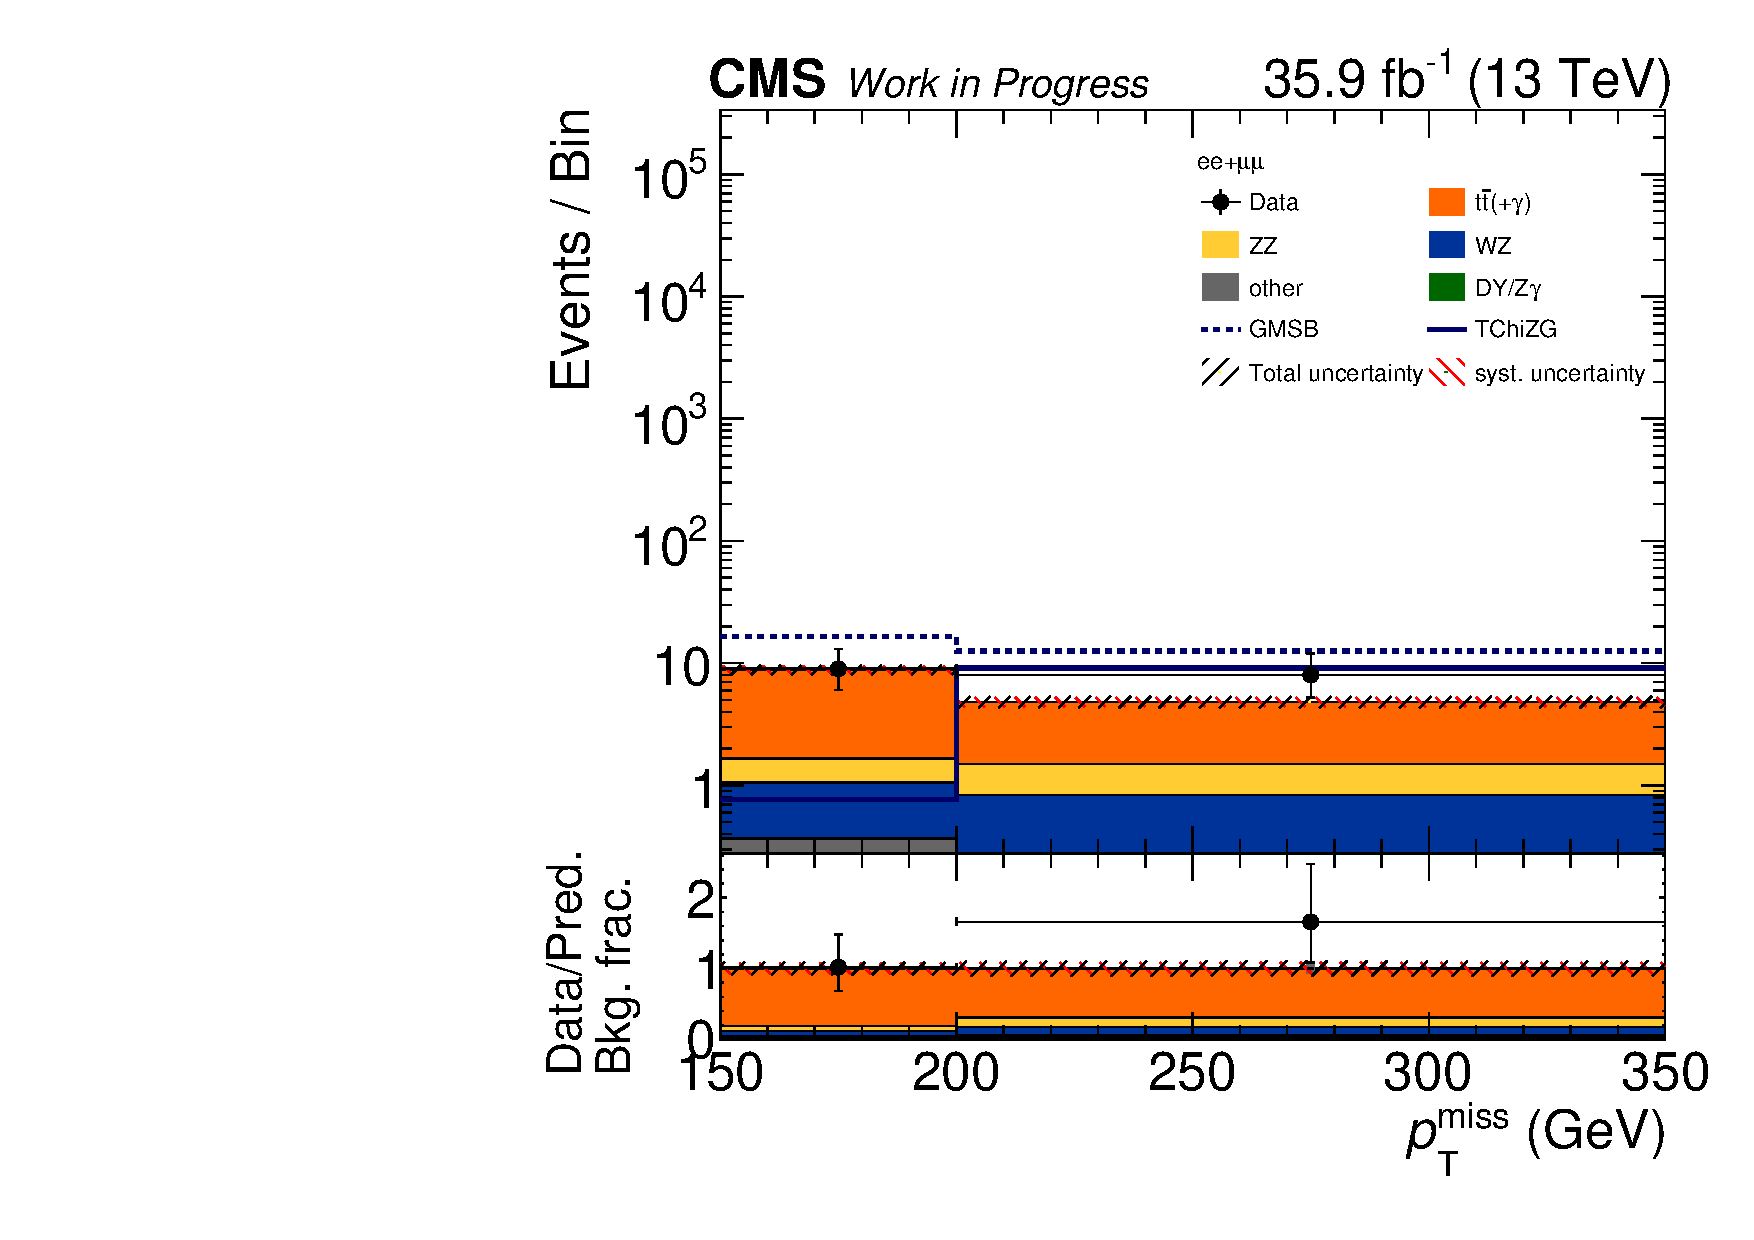
\includegraphics[width=\pairwidth]{figures/UnblindingPlots/final_MC_log}
 \caption{Comparison between final prediction and observation with statistical and systematic uncertainties in the signal region. Two signal expectations for the TChiZg model with $m(NLSP)=600\GeV$ and the GMSB model with $m(\tilde{W})=290\GeV$ and $m(\tilde{B})=205\GeV$ are also shown.}
 \label{fig:result}
\end{figure}
The number of background and observed events together with their total uncertainties are given also in \refTab{tab:results}. The total background uncertainties are obtained by adding the individual uncertainties quadratically. The statistical uncertainties on the measurement are calculated using $68\%$ confidence intervals of the Poissoin distribution with mean set to the observed yield.
\begin{table}[tbp]
 \centering
 \caption{Observed yields and final predicted background yields with the statistical and systematic uncertainties for each bin and background.}
 \normalsize
 \label{tab:results}
 \begin{tabular}{lllllll}
  $\ptmiss$      & \multicolumn{3}{l}{$150-200\GeV$} & \multicolumn{3}{l}{$200\GeV-\infinity$}                                                                  \\\hline
                 & yield                             & $\sigma_{stat}$                         & $\sigma_{syst}$ & yield & $\sigma_{stat}$    & $\sigma_{syst}$ \\\hline
  $\ttbar(\PGg)$ & 7.191                             & 0.316                                   & 0.664           & 3.320 & 0.229              & 0.395           \\
  DY/$\PZ(\PGg)$ & 0.152                             & 0.060                                   & 0.039           & 0.042 & 0.024              & 0.010           \\
  $\PW\PZ$       & 0.684                             & 0.081                                   & 0.063           & 0.579 & 0.076              & 0.054           \\
  $\PZ\PZ$       & 0.601                             & 0.019                                   & 0.052           & 0.667 & 0.020              & 0.061           \\
  Other          & 0.215                             & 0.215                                   & 0.191           & 0.214 & 0.214              & 0.108           \\\hline
  Total          & 8.843                             & 0.396                                   & 0.697           & 4.822 & 0.324              & 0.418           \\\hline
  Data           & 9                                 & $^{+4.11}_{-2.94}$                      & /               & 8     & $^{+3.95}_{-2.76}$ & /               \\\hline
 \end{tabular}
\end{table}


\section{Statistical interpretation}

\subsection{Limit calculation}

\subsection{Exclusion limits}

\subsubsection*{Limits on electroweak production of charginos and neutralinos}
\begin{figure}[tbp]
 \centering
 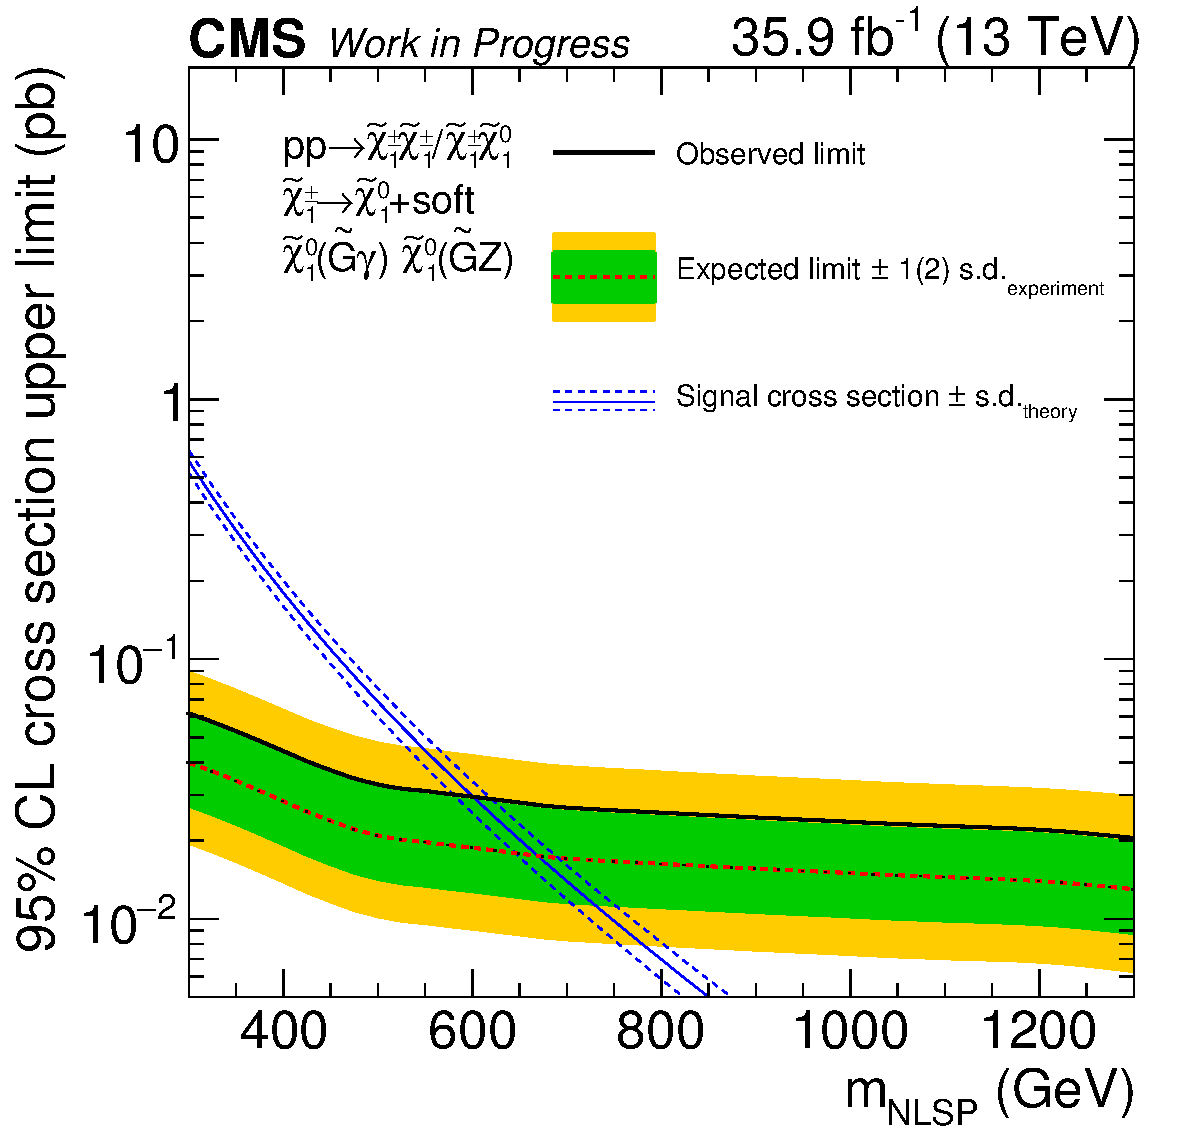
\includegraphics[width=\pairwidth]{figures/UnblindingPlots/TChiNG_limit2}
 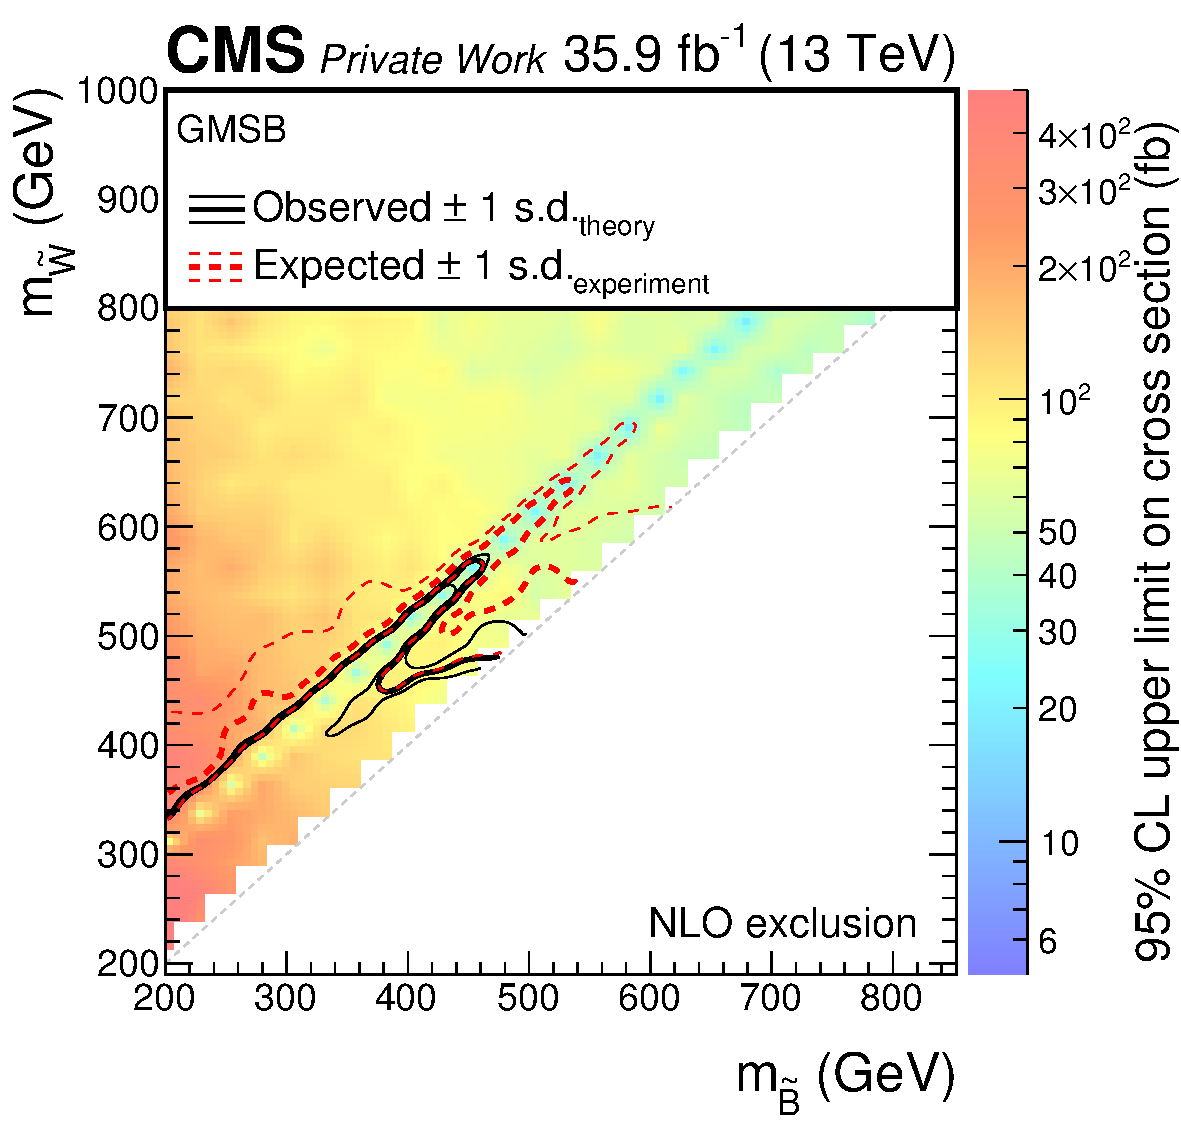
\includegraphics[width=\pairwidth]{figures/UnblindingPlots/GMSB_limits_XSEC2}
 \caption{Expected and observed upper limits for the TChiZG electroweak SMS (left) and the full GMSB model (right).}
 \label{fig:limitEWK}
\end{figure}

\subsubsection*{Limits on strong production of gluinos}

\begin{figure}[tbp]
 \centering
 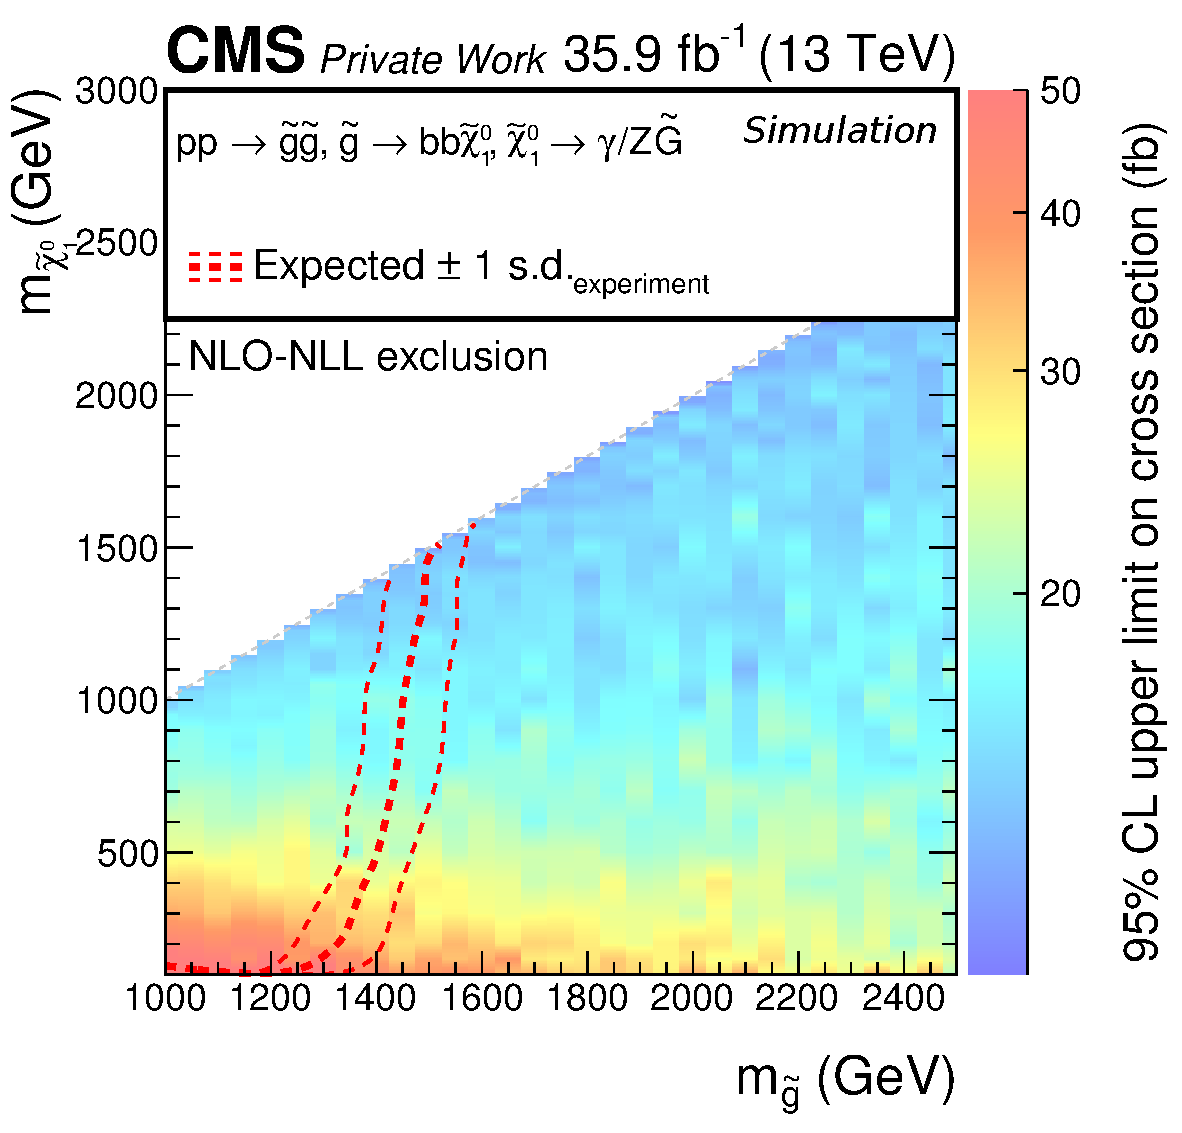
\includegraphics[width=\pairwidth]{UnblindingPlots/T5bbbbZg_limits_XSEC2}
 \caption{Expected and observed upper limits for the T5bbbbZG SMS with strong production.}
 \label{fig:limitStrong}
\end{figure}

\subsubsection*{Fit studies}\todo{rename}
